\documentclass{article}
%\documentclass{amsart}
%\documentclass{ws-m3as}
%\documentclass{m2an}
% SPRINGER
%\documentclass{svjour3}                    % onecolumn (standard format)
%\documentclass[smallextended]{svjour3}     % onecolumn (second format)
%\documentclass[twocolumn]{svjour3}         % twocolumn
%------------------------------------------------------------
% Defining page layout:
\pagestyle{plain} 
\setlength{\paperwidth}{210mm}
\setlength{\paperheight}{297mm} 
% on compte du bord du papier
\setlength{\hoffset}{-10mm}
\setlength{\voffset}{0mm} 
\setlength{\textwidth}{150mm}
\setlength{\textheight}{200mm} 
% marge gauche
\setlength{\evensidemargin}{0mm}
%\setlength\oddsidemargin{3cm}
% entete
\setlength{\topmargin}{0mm} 
%\setlength{\headheight}{0mm}
\setlength{\headsep}{10mm}
%pied de page
\setlength{\footskip}{20mm} 
% notes en marge droite
\setlength{\marginparsep}{0mm}
\setlength{\marginparwidth}{0mm} 
%\setlength\marginparpush{0cm}
% 
\parindent=0.5cm
\linespread{1.2}
% \textwidth 455pt \oddsidemargin 0pt \evensidemargin 0pt 
% \headsep 0pt \headheight 0pt \textheight 655pt \parskip 10pt
% \def\arraystretch{1.15}
% \renewcommand{\floatpagefraction}{0.75}
%------------------------------------------------------------
% Adding packages:
%\usepackage{url}
% mathematical symbols
\usepackage{latexsym}
\usepackage{amsmath}%
%\usepackage{amsfonts}%
\usepackage{amssymb}%
\usepackage{amsthm}
%\usepackage{dina4}
%\usepackage{mathtools} % (over/under)brackets
\usepackage{bm}
% graphical tools
\usepackage{graphicx}
%\usepackage{psfrag,psfig}
%\graphicspath{./fig/}
%\usepackage[pdftex]{graphicx}
%\usepackage{epsf}
%\usepackage{epsfig}
\usepackage[all]{xy}
\usepackage{hhline}
%\usepackage{exscale,cmmib57}
\usepackage{epic} %,eepic}% attention, dashline disparait avec eepic
%\usepackage{subfigure}
%\DeclareGraphicsExtensions{.jpg,.png,.pdf}
%\DeclareGraphicsRule{*}{mps}{*}{}
%\graphicspath{{fig/}}
% packages for layout
%\usepackage{geometry}
%\usepackage{afterpage}
%\usepackage{fullpage}
%\usepackage{fancyhdr}
% my additional package for fonts featuring
%\usepackage{mathptmx}      % SPRINGER use Times fonts if available on your TeX system
\usepackage[english]{babel}
%\usepackage[francais,english]{babel}
\usepackage[latin1]{inputenc}
\usepackage[T1]{fontenc}
%\usepackage[cyr]{aeguill} % guillemets
% my additional package for showing the labels
%\usepackage{showkeys}
%\usepackage[notref,notcite]{showkeys}
%\usepackage{showlabels}
%\usepackage{showtags}
%\usepackage{drafcopy}
%\usepackage{float}
\usepackage{enumerate} % to control the display of the enumeration counter
\usepackage{tikz}
\usepackage{enumitem}
\usetikzlibrary{shapes}
%------------------------------------------------------------
% Counters
%\newcounter{qn}[section]
%------------------------------------------------------------

%\smartqed  % SPRINGER flush right qed marks, e.g. at end of proof
% Theorem like environments
\newtheorem{theorem}{Theorem}
\theoremstyle{plain}
\newtheorem{acknowledgement}{Acknowledgement}
\newtheorem{algorithm}{Algorithm}
\newtheorem{axiom}{Axiom}
%\newtheorem{case}{Case}
%\newtheorem{claim}{Claim}
%\newtheorem{conclusion}{Conclusion}
%\newtheorem{condition}{Condition}
%\newtheorem{conjecture}{Conjecture}
\newtheorem{corollary}{Corollary}
%\newtheorem{criterion}{Criterion}
\newtheorem{definition}{Definition}
\newtheorem{example}{Example}
%\newtheorem{exercise}{Exercise}
\newtheorem{lemma}{Lemma}
\newtheorem{notation}{Notation}
\newtheorem{problem}{Problem}
\newtheorem{proposition}{Proposition}
\newtheorem{remark}{Remark}
%\newtheorem{solution}{Solution}
\newtheorem{summary}{Summary}
\numberwithin{equation}{section} % counter !!!!!!!
%\newtheorem{theorem}{Theorem}[section]
%\newtheorem{lemma}{Lemma}[section]
%\newtheorem{proposition}{Proposition}[section]
%\newtheorem{assumption}{Assumption}[section]
%\newtheorem{corollary}{Corollary}[section]
%\newtheorem{definition}{Definition}[section]
%\newtheorem{conjecture}{Conjecture}[section]
%\newtheorem{problem}{Problem}[section]
%\newtheorem{remark}{Remark}[section]
\newcommand\beq{\begin{equation}}
\newcommand\eeq{\end{equation}}
\renewcommand{\emph}{\textbf}
%\renewcommand{\emph}[1]{{\large \slshape #1}}
%------------------------------------------------------------
%------------------------------------------------------------
% Delimiters, norms, inner products...:
%
\newcommand{\brk}[1]{\left(#1\right)}          % \brk{.}     => (.)
\newcommand{\E}[1]{\mathbb{E}\brk{#1}}
\newcommand{\V}[1]{\mathbb{V}\brk{#1}}
\def\E{\mathbb{E}}
\def\V{\mathbb{V}}
\newcommand{\Brk}[1]{\left[#1\right]}          % \Brk{.}     => [.]
\newcommand{\BRK}[1]{\left\{#1\right\}}        % \BRK{.}     => {.}
\newcommand{\Average}[1]{\left<#1\right>}      % \Average{.} => <.>
\newcommand{\mean}[1]{\overline{#1}}           % \mean{.}
\newcommand{\Abs}[1]{\left| #1 \right|}        % \Abs{.}     => |.|
\newcommand{\Scal}[2]{\left(#1,#2\right)}      % \Scal{.}    => (.;.)
\newcommand{\Norm}[1]{\left\| #1 \right\|}     % \Norm{.}    => ||.||
\newcommand{\mymat}[1]{\begin{pmatrix} #1 \end{pmatrix}}
\newcommand{\jump}[1]{[\![#1]\!]}
%
%------------------------------------------------------------
% Special characters and shortcuts:
%
% my constants and parameters
\newcommand{\dd}{\frac{d(d+1)}{2}}
\newcommand{\dt}{\Delta t}
\newcommand{\Wi}{{\text{Wi}}}
\renewcommand{\Re}{{\text{Re}}}
\newcommand{\Ma}{{\text{Ma}}}
\newcommand{\Ra}{{\text{Ra}}}
\newcommand{\Fr}{{\text{Fr}}}
\renewcommand{\Pr}{{\text{Pr}}}
\newcommand{\Gr}{{\text{Gr}}}
\newcommand{\e}{\varepsilon}
\newcommand{\D}{\mathcal{D}}
\newcommand{\DD}{\mathrm{D}}
\newcommand{\f}{\boldsymbol{f}}
\newcommand{\I}{\boldsymbol{I}}
\newcommand{\xx}{\boldsymbol{x}}
\newcommand{\bolda}{\boldsymbol{a}}
\newcommand{\boldb}{\boldsymbol{b}}
\newcommand{\bzero}{{\boldsymbol{0}}}
\def\bn{\boldsymbol n}
\def\bN{\boldsymbol N}
\def\J{\boldsymbol J}
\newcommand{\NN}{\mathcal{N}}
% my limits
\renewcommand{\to}{\rightarrow}
\newcommand{\To}{\longrightarrow}
% my operators
\renewcommand{\div}{\operatorname{div}}
\newcommand{\curl}{\operatorname{curl}}
\newcommand{\tr}{\operatorname{tr}}
\newcommand{\range}{\operatorname{Range}}
\newcommand{\spn}{\operatorname{Span}}
\newcommand{\dist}{\operatorname{dist}}
\newcommand{\grad}{\boldsymbol{\nabla}}
\newcommand{\pd}[2]{\frac{\partial#1}{\partial#2}}
\newcommand{\deriv}[2]{\frac{d#1}{d#2}}
\newcommand{\pdd}[2]{\frac{\partial^2#1}{\partial#2^2}}
\newcommand{\pds}[1]{\partial_{#1}}
\newcommand{\pdds}[2]{\partial^2_{#1#2}}% my integrals
\newcommand{\intd}{\int_\D}
%\renewcommand{\liminf}[1]{\underset{#1}{\operatorname{liminf}}}
% my spaces
\newcommand{\N}{\mathbb{N}}
\newcommand{\R}{\mathbb{R}}
\newcommand{\RS}{\mathbb{R}^{d \times d}_S}
\newcommand{\RSPD}{\mathbb{R}^{d \times d}_{SPD}}
\newcommand{\PP}{\mathbb{P}}
\newcommand{\QQ}{\mathbb{Q}}
% \def\U{\mathrm{W}}  % !! \V does not always compile !!
% \def\Uz{\mathrm{V}}
\def\U{\mathrm{U}}
\def\V{\mathcal{V}}
\def\V{\mathrm{V}}
\def\H{\mathrm{H}}
\def\W{\mathrm{W}}
\def\Q{\mathrm{Q}}
\def\S{\mathrm{S}}
\def\SPD{\S_{PD}}
\def\Uh{\mathrm{W}_h}
\def\Uhz{\mathrm{V}_h}
\def\Vhzero{\mathrm{V}_{h}^0}
\def\Vhone{\mathrm{V}_{h}^1}
\def\Qh{\mathrm{Q}_h}
\def\Sh{\mathrm{S}_h}
\def\Shzero{\mathrm{S}_h^0}
\def\Shone{\mathrm{S}_h^1}
\def\ShonePD{\mathrm{S}_{h,PD}^1}
% my norms
\newcommand{\NormW}[3]{\|#1\|_{#2,#3}}
\newcommand{\NormH}[2]{\|#1\|_{#2}}
\newcommand{\NormLinf}[1]{\|#1\|_{L^\infty}}
\newcommand{\NormLone}[1]{\|#1\|_{L^1}}
\newcommand{\NormLtwo}[1]{\|#1\|_{L^2}}
\newcommand{\NormC}[1]{\|#1\|_{C^0}}
\newcommand{\NormHolder}[3]{\|#1\|_{C^{#2,#3}}}
\newcommand{\SemiNormHolder}[2]{|#1|_{C^{#2}}}
% my fluid variables
\newcommand{\str}{{\boldsymbol{\tau}}}
\newcommand{\strs}{{\boldsymbol{\sigma}}}
\newcommand{\bu}{{\boldsymbol{u}}}
\newcommand{\bv}{\boldsymbol{v}}
\newcommand{\bw}{\boldsymbol{w}}
\newcommand{\bz}{\boldsymbol{z}}
\newcommand{\be}{\boldsymbol{e}}
\newcommand{\bg}{\boldsymbol{g}}
\newcommand{\vort}{{\boldsymbol{\omega}}}
\newcommand{\gbu}{{\grad\bu}}
\newcommand{\gbv}{{\grad\bv}}
% \newcommand{\Dbu}{{\frac12(\gbu+\gbu^T)}}
% \newcommand{\Dbv}{{\frac12(\gbv+\gbv^T)}}
\def\Dbu{\boldsymbol{D}(\bu)}
\def\Dbv{\boldsymbol{D}(\bv)}
\newcommand{\bphi}{\boldsymbol{\phi}}
\newcommand{\bpsi}{\boldsymbol{\psi}}
\newcommand{\bchi}{\boldsymbol{\chi}}
\newcommand{\bLambda}{\boldsymbol{\Lambda}}
\newcommand{\bXi}{\boldsymbol{\Xi}}
\newcommand{\bxi}{\boldsymbol{\xi}}
\newcommand{\bvarsigma}{\boldsymbol{\varsigma}}
% my space-discretised variables
\newcommand{\buh}{\bu_h}
\newcommand{\bvh}{\bv_h}
\def\Dbuh{\boldsymbol{D}(\buh)}
\def\Dbvh{\boldsymbol{D}(\bvh)}
\newcommand{\ph}{p_h}
\newcommand{\qh}{q_h}
\newcommand{\gbuh}{\grad\bu_h}
\newcommand{\strh}{\strs_h}
% my regularized variables
\newcommand{\prd}{p_{\delta}}
\newcommand{\paL}{p_{\alpha}^L}
\newcommand{\padL}{p_{\alpha,\delta}^L}
\newcommand{\paorL}{p_{\alpha}^{(L)}}
\newcommand{\padorL}{p_{\alpha,\delta}^{(L)}}
\newcommand{\bud}{\bu_\delta}
\newcommand{\gbud}{\grad\bu_\delta}
\newcommand{\strd}{\strs_\delta}
\newcommand{\bua}{\bu_\alpha}
\newcommand{\gbua}{\grad\bu_\alpha}
\newcommand{\stra}{\strs_\alpha}
\newcommand{\budL}{\bu_{\delta,L}}
\newcommand{\buaL}{\bu_{\alpha}^{L}}
\newcommand{\buadL}{\bu_{\alpha,\delta}^{L}}
\newcommand{\buaorL}{\bu_{\alpha}^{(L)}}
\newcommand{\buadorL}{\bu_{\alpha,\delta}^{(L)}}
\newcommand{\gbudL}{\grad\bu_{\delta,L}}
\newcommand{\gbuaL}{\grad\bu_{\alpha}^{L}}
\newcommand{\gbuadL}{\grad\bu_{\alpha,\delta}^{L}}
\newcommand{\gbuaorL}{\grad\bu_{\alpha}^{(L)}}
\newcommand{\gbuadorL}{\grad\bu_{\alpha,\delta}^{(L)}}
\newcommand{\strdL}{\strs_{\delta,L}}
\newcommand{\straL}{\strs_{\alpha}^{L}}
\newcommand{\stradL}{\strs_{\alpha,\delta}^{L}}
\newcommand{\straorL}{\strs_{\alpha}^{(L)}}
\newcommand{\stradorL}{\strs_{\alpha,\delta}^{(L)}}
% my space-discretised regularized variables
\newcommand{\buhd}{\bu_{\delta,h}}
\newcommand{\gbuhd}{\grad\bu_{\delta,h}}
\newcommand{\strhd}{\strs_{\delta,h}}
\newcommand{\buhdL}{\bu_{\delta,L,h}}
\newcommand{\gbuhdL}{\grad\bu_{\delta,L,h}}
\newcommand{\stradh}{\strs_{\alpha,\delta,h}}
% my space-discretised regularized extra-diffusive variables
\newcommand{\buhda}{\bu_{\alpha,\delta,h}}
\newcommand{\gbuhda}{\grad\bu_{\alpha,\delta,h}}
\newcommand{\strhda}{\strs_{\alpha,\delta,h}}
\newcommand{\buhdLa}{\bu_{\alpha,\delta,h}}
\newcommand{\gbuhdLa}{\grad\bu_{\alpha,\delta,h}}
\newcommand{\strhdLa}{\strs_{\alpha,\delta,h}}
\newcommand{\buhLa}{\bu_{\alpha,h}}
\newcommand{\gbuhLa}{\grad\bu_{\alpha,h}}
\newcommand{\strhLa}{\strs_{\alpha,h}}
% my time-discretised variables
\newcommand{\strn}{\strs^n}
\newcommand{\strnp}{\strs^{n+1}}
\newcommand{\bun}{\bu^n}
\newcommand{\bunp}{\bu^{n+1}}
\newcommand{\pn}{p^n}
\newcommand{\qn}{q^n}
\newcommand{\Ln}{\Lambda^n}
\newcommand{\Lnp}{\Lambda^{n+1}}
% my space-and-time-discretised variables
\newcommand{\buhn}{\bu_h^n}
\newcommand{\buhnp}{\bu_h^{n+1}}
\newcommand{\buhnm}{\bu_h^{n-1}}
\def\Dbuhnm{\boldsymbol{D}(\buhnm)}
\def\Dbuhn{\boldsymbol{D}(\buhn)}
\def\Dbuhnp{\boldsymbol{D}(\buhnp)}
\newcommand{\strhnp}{\strs_h^{n+1}}
\newcommand{\strhnpp}{\strs_h^{n+1,+}}
\newcommand{\strhnpm}{\strs_h^{n+1,-}}
\newcommand{\strhn}{\strs_h^n}
\newcommand{\phn}{p_h^n}
\newcommand{\phnp}{p_h^{n+1}}
\newcommand{\gbuhnp}{\gbu_h^{n+1}}
\newcommand{\gbuhn}{\gbu_h^n}
%%%%%%%%%%%%%%%%%%%%%%%%%%%%%%%%
%\usepackage{verbatim}
%%
%% Pour activer les commentaires
%%
%%
\newcommand{\comment}[1]{ { ***~{\bf #1}~***}}
%%
%% Pour desactiver les commentaires
%%
% \newcommand{\comment}[1]{ }
%%%%%%%%%%%%%%%%%%%%%%%%%%%%%%%%
%--------------------------------------------------------
% \journalname{myjournal} % SPRINGER Insert the name of "your journal"

\begin{document}

\title{Sch\'emas utilis\'es}

%\thanks{Grants or other notes
%about the article that should go on the front page should be
%placed here. General acknowledgments should be placed at the end of the article.} % SPRINGER
%\subtitle{..} % SPRINGER
%\titlerunning{Reduced-Basis : Uncertain coefficients in elliptic PDEs}% SPRINGER

\author{Pierre Marchand
%S\'ebastien Boyaval
% \footnote{
% Laboratoire d'hydraulique Saint-Venant,\\ Universit\'e Paris-Est
% (Ecole des Ponts ParisTech) EDF R\&D,\\ 6 quai Watier, 78401 Chatou Cedex, France
% \\[2mm]       
% sebastien.boyaval@enpc.fr
% \\[2mm]
% Present address: EPFL
%}
}
%\authorrunning{Short form of author list} % SPRINGER if too long for running head

% \begin{history}
% \received{}
% \revised{}
% \end{history}
%\date{Received: date / Accepted: date} % SPRINGER
%\date{\today}

\maketitle
%\begin{abstract}
%We investigate the capabilities of the ALE method for the numerical simulation of gravity waves.
% \PACS{PACS code1 \and PACS code2 \and more}
% \subclass{MSC code1 \and MSC code2 \and more}
% \keywords{Finite element method, convergence analysis, existence of weak solutions.}%
%\end{abstract}

%\subjclass{} %

% \keywords{Finite element method, convergence analysis, existence of weak solutions.}%
% \ccode{AMS Subject Classification: 35Q30, 65M12, 65M60, 76A10, 76M10, 82D60}

%\tableofcontents

%\begin{acknowledgements}
%If you'd like to thank anyone, place your comments here
%and remove the percent signs.
%\end{acknowledgements}
\section{Introduction}

On se proprose de mettre en avant la diff\'erence entre la mod\`ele potentiel lin\'eaire et le probl\`eme de Stokes, et ceci, afin d'observer la partie vorticale ainsi que l'effet de la viscosit\'e.



\begin{center}
	\begin{tikzpicture}
		\tikzstyle{titre}=[draw,rectangle]
		\tikzstyle{equation}=[draw,rectangle]
		\tikzstyle{hypothese}=[draw,ellipse]
		\node[titre] (T1) at (0,1.7){Navier-Stokes};
		\node[equation] (NS) at (0,0)  {
			$
			\begin{array}{rcl}
   				\frac{\partial \bu}{\partial t}+ \bu \cdot \nabla \bu - \nu \Delta\bu+\frac{1}{\rho}\nabla p  =& \mathbf{g}  &\text{ pour -h}\leq z\leq \eta \\
   				\div (\bu) =& 0 &\text{ pour -h}\leq z\leq \eta \\
   				\bu \cdot \mathbf{n} =& 0 &  \text{ en }z=-h \\
   				-(p-p_0)\mathbf{n}+\mu (\nabla \bu + \nabla \bu^T)\cdot \mathbf{n} =& 0 & \text{ en }z=\eta \\
   				\frac{\partial \eta }{ \partial t} + u_x \frac{\partial \eta}{\partial x}  =& u_z & \text{ en }z=\eta
  				\end{array}
			$
		};
		\node[hypothese] (H1) at (-7.5,0){\'Ecoulement lin\'earis\'e};
		\node[titre] (T2) at (-7.5,-4.7){Stokes};
		\node[equation] (S) at (-7.5,-3)  {
			$
			\begin{array}{rcl}
   				\frac{\partial \bu}{\partial t} - \nu \Delta\bu+\frac{1}{\rho}\nabla p  =& \mathbf{g}  &\text{ pour -h}\leq z\leq \eta \\
   				\div (\bu) =& 0 &\text{ pour -h}\leq z\leq \eta \\
   				\bu \cdot \mathbf{n} =& 0 &  \text{ en }y=-h \\
   				-(p-p_0)\mathbf{n}+\mu (\nabla \bu + \nabla \bu^T)\cdot \mathbf{n} =& 0 & \text{ en }z=\eta \\
   				\frac{\partial \eta }{ \partial t} + u_x \frac{\partial \eta}{\partial x}  =& u_z & \text{ en }z=\eta
  			\end{array}
			$
		};
		\node[hypothese] (H2) at (0,-3){$\bu=\nabla \phi$};
		\node[titre] (T3) at (0,-7.8){\'Ecoulement potentiel visqueux};
		\node[equation] (PV) at (0,-6)  {
			$
			\begin{array}{rcl}
   				\frac{\partial \phi}{\partial t} +\frac{p-p_0}{\rho} +gz  =& 0  &\text{ pour -h}\leq z\leq \eta \\
   				\Delta \phi =& 0 &\text{ pour -h}\leq z\leq \eta \\
   				\nabla \phi \cdot \mathbf{n} =& 0 &  \text{ en }y=-h \\
   				-(p-p_0)\mathbf{n}+\mu (\nabla \bu + \nabla \bu^T)\cdot \mathbf{n} =& 0 & \text{ en }z=\eta \\
   				\frac{\partial \eta }{ \partial t} + \frac{\partial \phi}{\partial x} \frac{\partial \eta}{\partial x}  =& \frac{\partial \phi}{\partial z} & \text{ en }z=\eta
  			\end{array}
			$
		};		
		\node[hypothese] (H3) at (-7.5,-6){$\nu=0$};
		\node[titre] (T4) at (-7.5,-10.8){\'Ecoulement potentiel};
		\node[equation] (P) at (-7.5,-9)  {
			$
			\begin{array}{rcl}
   				\frac{\partial \phi}{\partial t} +\frac{p-p_0}{\rho} +gz  =& 0  &\text{ pour -h}\leq z\leq \eta \\
   				\Delta \phi =& 0 &\text{ pour -h}\leq z\leq \eta \\
   				\nabla \phi \cdot \mathbf{n} =& 0 &  \text{ en }y=-h \\
   				p=&p_0 & \text{ en }z=\eta \\
   				\frac{\partial \eta }{ \partial t} + \frac{\partial \phi}{\partial x} \frac{\partial \eta}{\partial x}  =& \frac{\partial \phi}{\partial z} & \text{ en }z=\eta
  				\end{array}
			$
		};	
		\node[hypothese] (H4) at (0,-9){Lin\'earisation de la surface libre};			
		\node[titre] (T5) at (0,-13.75){Vague lin\'eaire};
		\node[equation] (LV) at (0,-12)  {
			$
			\begin{array}{rcl}
   				\Delta \phi =& 0 &\text{ pour -h}\leq z\leq \eta \\
   				\frac{\partial \phi}{\partial t} +g\eta  =& 0  & \text{ en }z=0 \\
   				\nabla \phi \cdot \mathbf{n} =& 0 &  \text{ en }z=-h \\
   				\frac{\partial \eta }{ \partial t} =& \frac{\partial \phi}{\partial z} & \text{ en }z=0\\
   				\frac{\partial \phi}{\partial t} +\frac{p-p_0}{\rho} +gz  =& 0  &\text{ pour -h}\leq z\leq 0 
  				\end{array}
			$
		};	
				
		
		\draw (T1)--(NS);
		\draw[-latex](NS)--(H1);
		\draw[-latex](H1)--(S) ;
		\draw (T2)--(S);
		\draw[-latex](S)--(H2) ;
		\draw[-latex](H2)--(PV);
		\draw (T3)--(PV);
		\draw[-latex](PV)--(H3);
		\draw[-latex](H3)--(P);
		\draw (T4)--(P);
		\draw[-latex](P)--(H4);
		\draw[-latex](H4)--(LV);
		\draw (T5)--(LV);
		
	\end{tikzpicture}
\end{center}
\section{Potentiel}

On consid\`ere le probl\`eme suivante :
\[
	\left\{
		\begin{array}{rcl}
   			\Delta \phi  =& 0  &\text{ dans }\Omega \\
   			\frac{\partial \phi }{ \partial z} =& 0 & \text{ en }z=-h \\
   			\frac{\partial \eta }{ \partial t} =& \frac{\partial \phi }{ \partial z} & \text{ en }z=0 \\
   			\frac{\partial \phi }{ \partial t} + g\eta =& 0 & \text{ en }y=0,
  		\end{array}
	\right.
\]

qui peut aussi s'\'ecrire de la fa\c con suivante : 

\[
	\left\{
		\begin{array}{rcl}
   			\Delta \phi  =& 0  &\text{ dans }\Omega \\
   			\frac{\partial \phi }{ \partial z} =& 0 & \text{ en }z=-h \\
   			\frac{\partial^2 \phi }{ \partial t^2} +g \frac{\partial \phi }{ \partial z}=& 0 & \text{ en }z=0 \\
  		\end{array}
	\right.
\]
On remarque qu'on peut trouver $\phi$ si on a sa valeur en $z=0$. On propose alors plusieurs sch\'emas avec $\varphi=\phi_{|z=0}$:
\begin{enumerate}
	\item On se donne ($\phi_{0}$,$\phi_{1}$) puis $\varphi_2=-g\Delta t \frac{\partial \varphi_1}{\partial y}+2\varphi_1-\varphi_0$
	\item On se donne ($\varphi_0,\eta_0$) puis $\varphi_1=-g \eta_0 \Delta t +\varphi_0$ et apr\`es $\eta_1=\eta_0+\Delta t \frac{\partial \varphi_1}{\partial y}$
	\item On se donne ($\varphi_0,\eta_0$) puis $\eta_1=\eta_0+\Delta t \frac{\partial \varphi_0}{\partial y}$ et apr\`es $\varphi_1=-g \eta_1 \Delta t +\varphi_0$
\end{enumerate}
Le premier sch\'ema semble assez peu stable tandis que les deux derniers semblent \'equivalents. Les deux derniers sch\'emas sont du type \textit{Euler symplectique} et comme notre problème admet une Hamiltonien pour la dynamique suivante :
\[
	\left\{	
		\begin{array}{rcl}
			\frac{\partial \varphi}{\partial t} =& -g\eta & \text{ en }z=0\\
			\frac{\partial \eta}{\partial t} =& \frac{\partial \phi}{\partial z} & \text{ en }z=0\\
		\end{array}
	\right.
\]
on peut observer qu'ils sont \'equivalents en pr\'ecision et qu'ils ont un bon comportement en temps long. Mais pour garder la structure Hamiltonienne et profiter des avantages de ces sch\'emas, il faut retravailler la condition dynamique car elle fait appara\^itre une d\'eriv\'ee en $\phi$. Celle-ci implique une erreur d'interpolation pour r\'ecup\'erer des \'el\'ements finis du m\^eme ordre que $\eta$ et $\phi$. Pour \'eviter cela, on va r\'esoudre la condition dynamique faiblement. Soit $\hat{w}\in \H^1(\Omega)$ et $w$ sa trace. On a alors en appliquant la formule de Stokes et en utilisant le fait que $\Delta \phi =0$ :
\begin{align*}
	\left(\frac{\partial \eta}{\partial t},w\right)_{\Gamma_0}=&\left(\frac{\partial \phi}{\partial z},w\right)_{\Gamma_0}\\
	\left(\frac{\partial \eta}{\partial t},w\right)_{\Gamma_0}=&\int_{\partial \Omega}(\nabla \phi \cdot \mathbf{n}) w   \\
	\left(\frac{\partial \eta}{\partial t},w\right)_{\Gamma_0}=&\int_{\Omega} \div(\nabla \phi \mbox{ }\hat{w})   \\
	\left(\frac{\partial \eta}{\partial t},w\right)_{\Gamma_0}=&\int_{\Omega} \nabla \phi \cdot \nabla \hat{w}.
\end{align*}
On obtient une formulation variationelle de la condition dynamique ad\'equate aux \'el\'ements finis. Seul les termes \`a la surface libre nous int\'eressent, il faut donc extraire de la matrice de masse la sous matrice correspondant aux noeuds \`a la surface libre pour le terme de droite et supprimer les lignes correspondant \`a ces derniers dans la matrice de rigidit\'e. Toujours dans l'id\'ee de profiter de la structure Hamiltonienne du probl\`eme, on propose aussi un sch\'ema du type \textit{velocity verlet} qui \`a l'avantage d'\^etre d'ordre 2 : 
 
\begin{enumerate}[resume]
	\item On se donne ($\varphi_0,\eta_0$) puis $\eta_{\frac{1}{2}}=\eta_0+\frac{\Delta t}{2} \frac{\partial \varphi_0}{\partial y}$ puis $\varphi_1=-g \eta_{\frac{1}{2}} \Delta t +\varphi_0$ et enfin $\eta_{1}=\eta_{\frac{1}{2}}+\frac{\Delta t}{2} \frac{\partial \varphi_1}{\partial y}$.
\end{enumerate}


\section{Stokes}
\subsection{\`A surface libre lin\'earis\'ee}



\subsection{\`A surface libre}
On s'int\'eresse au probl\`eme suivant :
\[
	\left\{
			\begin{array}{rcl}
   				\frac{\partial \bu}{\partial t} - \nu \Delta\bu+\frac{1}{\rho}\nabla p  =& \mathbf{g}  &\text{ pour -h}\leq z\leq \eta \\
   				\div (\bu) =& 0 &\text{ pour -h}\leq z\leq \eta \\
   				\bu \cdot \mathbf{n} =& 0 &  \text{ en }y=-h \\
   				-(p-p_0)\mathbf{n}+\mu (\nabla \bu + \nabla \bu^T) =& 0 & \text{ en }z=\eta \\
   				\frac{\partial \eta }{ \partial t} + u_x \frac{\partial \eta}{\partial x}  =& u_z & \text{ en }z=\eta
  			\end{array}
	\right.
\]
qui, a priori, doit comporter une composante verticale contrairement au cas uniquement potentiel. On r\'esout ce probl\`eme \`a l'aide d'une m\'ethode ALE avec deux sch\'emas num\'eriques possibles. On note $\mathbf{X}^{n}$, la position des noeuds, $\mathbf{V}^{n}$, la vitesse des noeuds, $\mathbf{U}^{n}$, la vitesse du fluide aux noeuds, $\mathbf{P}^{n}$, la valeur de la pression aux noeuds , $M$, la matrice de masse, $R$, la matrice de rigidit\'e qui inclue en plus les termes li\'es \`a la vitesse du maillage, $F$, le vecteur force, $L$, le probl\`eme v\'erifi\'e par la vitesse du maillage et $B$, le vecteur associé aux conditions de bords, $G$, la matrice li\'ee aux termes couplant vitesse et pression, et $D$, la matrice li\'ee \`a l'incompressibilit\'e du fluide. On notera $D_2$, l'op\'erateur tel que $D_2 f^{n+1}=\frac{3}{2}f^{n+1}-2f^{n}+\frac{1}{2}f^{n-1}$.
\begin{enumerate}

	\item Version conservative
	\begin{itemize}
		\item Initialisation :  ($\Omega_0$,$\bu_0$,$p_0$)
		\item  $L(\mathbf{X}^{n})\mathbf{V}^{n}=0$\\
		On en d\'eduit la vitesse du maillage.
		\item $\mathbf{X}^{n+1}=\mathbf{X}^{n}+\Delta t \mathbf{V}^{n}$\\
		On en d\'eduit $\Omega_{n+1}$, on va maintenant boucler sur i avec $\mathbf{V}^{n+1}_0=\mathbf{V}^n$.
		\item  $M(\mathbf{X}^{n+1})\frac{1}{\Delta t}D_2 \mathbf{U}^{n+1}_i=R(\mathbf{X}^{n+1},\mathbf{V}^{n+1}_i)\mathbf{U}^{n+1}_i+G(\mathbf{X}^{n+1})\mathbf{P}^{n+1}_i+F(\mathbf{X}^{n+1},t_{n+1})$ et $D(\mathbf{X}^{n+1})\mathbf{U}^{n+1}_i=0$\\
		\item $L(\mathbf{X}^{n+1})\mathbf{V}^{n+1}_{i+1}=B(\mathbf{U}^{n+1}_i)$\\
		On regarde la diff\'erence en norme $\mathrm{L}_2$ sur la vitesse pour tester la convergence, et si cela \`a converger, on passe \`a l'\'etape suivante.
	\end{itemize}	
	
	\item Version non conservative
	
	\begin{itemize}
		\item Initialisation : ($\Omega_0$,$\bu_0$,$p_0$) et ($\Omega_1$,$\bu_1$,$p_1$)
		\item $\hat{\mathbf{U}}^{n+1}$=2$\mathbf{U}^{n}$-$\mathbf{U}^{n-1}$\\
		Avec la formule (BDF2 extrapol\'ee mais je n'ai toujours pas compris le rapport) : $\hat{f}_{n+1}=2f_n-f_{n-1}$, on obtient une vitesse $\hat{\mathbf{U}}^{n+1}$ d\'efinie sur un domaine $\hat{\Omega}^{n+1}$ avec $\hat{\mathbf{X}}^{n+1}$.
		\item $L(\hat{\mathbf{X}}^{n+1})\mathbf{V}^{n+1}=B(\hat{\mathbf{U}}^{n+1})$\\
		On en d\'eduit la vitesse du maillage en n+1.
		\item $\frac{1}{\Delta t}D_2 \mathbf{X}^{n+1}=\mathbf{V}^{n+1}$ \\
		On en d\'eduit $\Omega^{n+1}$
		\item $M(\mathbf{X}^{n+1})\frac{1}{\Delta t}D_2 \mathbf{U}^{n+1}=R(\mathbf{X}^{n+1},\mathbf{V}^{n+1})\mathbf{U}^{n+1}+G(\mathbf{X}^{n+1})\mathbf{P}^{n+1}+F(\mathbf{X}^{n+1},t_{n+1})$ et $D(\mathbf{X}^{n+1})\mathbf{U}^{n+1}=0$\\
		On r\'esout le probl\`eme au pas de temps n en calculant la vitesse et la pression.
	\end{itemize}

\end{enumerate}

%\bibliographystyle{ws-m3as}
\bibliographystyle{amsplain}
%\bibliographystyle{plain}
%\bibliographystyle{plain}
%\bibliographystyle{spbasic}      % basic style, author-year citations
%\bibliographystyle{spmpsci}      % mathematics and physical sciences
%\bibliographystyle{spphys}       % APS-like style for physics
%\bibliography{/home/sebastien/Bureau/Z_boyaval/database/myrefs} % portable
\bibliography{/local00/home/SB03743S/Desktop/Z/database/myrefs} % EDF

\end{document}
